\documentclass{controle}
\usepackage{main}

\title{Contrôle n°3 : Fonctions}
\author{Seconde 3}
\date{7 Janvier 2026}

\begin{document}
\maketitle
\instructions[autorisée]
\begin{questions}
\titledquestion{Univers et événements}[5]
Dans une urne opaque, on installe des boules colorées et numérotées :
\begin{itemize}
\item Trois boules rouges numérotées de $1$ à $3$;
\item Deux boules bleues numérotées $1$ et $3$;
\item Deux boules vertes numérotées $2$ et $3$ 
\end{itemize}
\begin{parts}
\part[1] On tire une boule au hasard, et on regarde son numéro ($1$; $2$ ou $3$) \textbf{ET} sa couleur ($R$;$G$ ou $B$). Recopier et compléter l'univers $\Omega$ de cette expérience aléatoire :
\begin{equation*}
\Omega = \set{R3; B3; V3; \dots}
\end{equation*}
\part[1] On pose deux événements d'$\Omega$ :
\begin{itemize}
\item $R$ : \og La boule tirée est rouge \fg
\item $T$ : \og La boule tirée affiche $3$ \fg
\end{itemize}
Donner $R$ et $T$ sous forme d'ensemble.
\part[3] Décrire les événements suivants à l'aide d'une phrase en français sous forme d'ensemble :
\begin{subparts}
\subpart $R \cap T$
\subpart $R \cup T$
\subpart $\overbar{R}$
\end{subparts}
\end{parts}
\titledquestion{Décollage imminent}[7,5]
Des étudiants lancent un prototype de fusée. Ils ne souhaitent pas voir leur création se briser à l'atterissage, ce qui se produit si le prototype dépasse les \qty{4}{\meter} durant son envol. On note $h(t)$ la hauteur (en mètres) atteinte par la fusée en fonction du temps $t$ (en secondes). L'allure de la courbe $\mathcal{C}_h$ représentative de $h$ est donnée ci-contre
:
\begin{center}
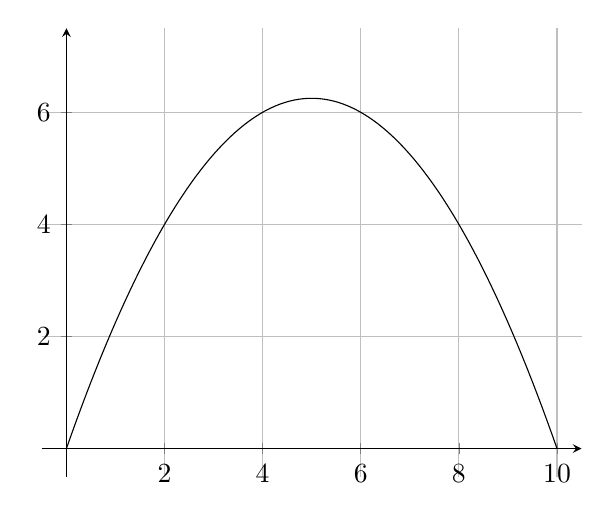
\begin{tikzpicture}
\begin{axis}[
  xmin=-0.5,
  xmax=10.5,
  ymin=-0.5,
  ymax=7.5,
  axis lines=center,
  grid=major
]
\addplot[
  domain=0:10,
  samples=100,
  ]
{-x*(x-10)/4};
\end{axis}
\end{tikzpicture}
\end{center}
\begin{parts}
\part[0,5] Donner l'image de $4$ par la fonction $h$.
\part[1] À quel instant la fusée atterit-elle ?
\part[1] Résoudre l'équation $h(t) = 6$. On donnera notamment l'ensemble $S$ des solutions.
\part[1,5] Résoudre graphiquement l'inéquation $h(t) \geq 4$. On donnera notamment l'ensemble $S$ des solutions de cette inéquation.
\part[0,5] La fusée se casse-t-elle à l'atterissage ?
\part[3] Le groupe décide de changer la puissance de son moteur pour l'empêcher de se casser. L'expression de la fonction $h$ est donnée par
\begin{equation*}
h(t) = a(t^2 - 10t)
\end{equation*}
avec $a$ un nombre correspondant à la puissance du moteur.
\begin{subparts}
\subpart[1] On admet que $h(5)$ correspond à l'altitude maximale atteinte par la fusée. Si on suppose que $a = 0.1$, quelle est l'altitude maximale de la fusée ?
\subpart[2] Pour quelle valeur de $a$ la fusée a pour altitude maximale \qty{4}{\meter} ?
\end{subparts}
\end{parts}
\titledquestion{Équations et Inéquations}[7,5]
\end{questions}
\end{document}